\documentclass[a4paper,12pt]{article}

\usepackage[14pt]{extsizes}
\usepackage{cmap}					% поиск в PDF
\usepackage{mathtext} 				% русские буквы в формулах
\usepackage[T2A]{fontenc}			% кодировка
\usepackage[utf8]{inputenc}			% кодировка исходного текста
\usepackage[english,russian]{babel}	% локализация и переносы
\usepackage{graphicx}
\usepackage{geometry}
\usepackage{amsmath}
\usepackage[table]{xcolor}
\setlength\extrarowheight{2pt}


\geometry{verbose, a4paper, tmargin=2cm, bmargin=2cm, lmargin=3cm, rmargin=2cm}
\author{Vysotsky Maxim}
\title{Отчёт}
\date{2022}

\begin{document}
	\begin{titlepage}
		\begin{center}
			{Министерство науки и высшего образования Российской Федерации
				НОВОСИБИРСКИЙ НАЦИОНАЛЬНЫЙ ИССЛЕДОВАТЕЛЬСКИЙ
				ГОСУДАРСТВЕННЫЙ УНИВЕРСИТЕТ (НГУ)}
		\end{center}
		\begin{center}
			{Физический факультет}
		\end{center}
		
		
		\vspace{8cm}
		{
			\begin{center}
				{\bf Лабораторная работа №4.2}\\
				Мостовые методы измерения сопротивлений
			\end{center}
		}
		\vspace{2cm}
		\begin{flushright}
			{Руководитель:\\ Старший преподаватель\\
				Яцких А. А.\\
				Работу выполнил:\\
				Высоцкий М. Ю.\\
				\vspace{0.2cm}
				гр. 24301}
		\end{flushright}
		\vspace{3cm}
		\begin{center}
			Новосибирск, 2024
		\end{center}
	\end{titlepage}

\section{Теоретическое введение}
\textbf{Цель работы:} Изучение мостовых методов измерения электрических сопротивлений, принципов работы одинарного и двойного мостов, измерения температуры датчиками сопротивления.

    Мостами называются приборы, предназначенные для измерения сопротивлений
методом сравнения. Для измерения сопротивлений более 50 Ом применяют одинарный мост – мост Уитстона. При измерении малых сопротивлений применяют двойной мост – мост Томпсона.

Схема одинарного моста приведена ниже. По сути, он представляет собой два делителя напряжения, включенных параллельно. Сопротивления R1, R2 и R являются элементами моста и их значения известны. Сопротивление Rx - это неизвестное (измеряемое) сопротивление. Одно из сопротивлений моста (по схеме - это сопротивление R) можно изменять в широких пределах, меняя, тем самым, коэффициент деления правого по схеме делителя напряжения, и, следовательно, потенциал в точке В. В процессе измерений мы меняем R в ту или иную сторону, добиваясь нулевых показаний индикатора Г, включенного
в измерительную диагональ моста – уравновешиваем мост. В этот момент потенциалы в точках А и В равны:
\begin{equation}
    \frac{UR_x}{R_x+R_1} = \frac{UR}{R+R_2}
\end{equation}
откуда
\begin{equation}
    R_x = R \frac{R_1}{R_2}
\end{equation}
Поскольку значения всех сопротивлений в правой части этого выражения нам известны, мы можем рассчитать $R_x$.


\begin{figure}[h!]
	\begin{center}
		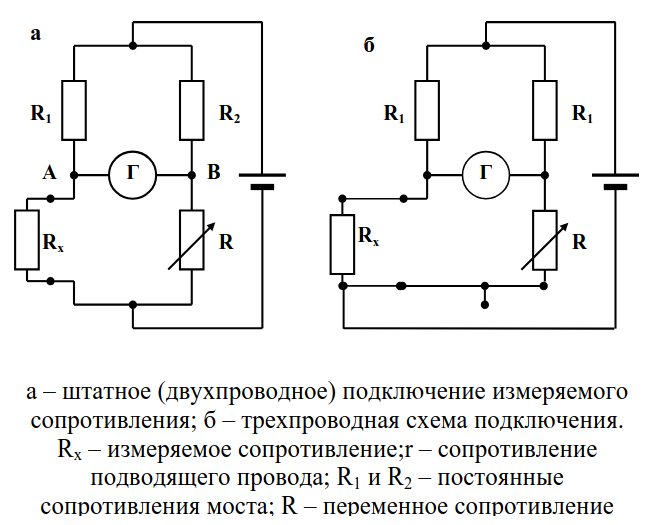
\includegraphics[scale=0.8]{scheme_1.png}
	\end{center}
	\caption{Мост Уитстона.}
\end{figure}
\clearpage

Далее - двойной мост, мост Томпсона.
\begin{figure}[ht!]
	\begin{center}
		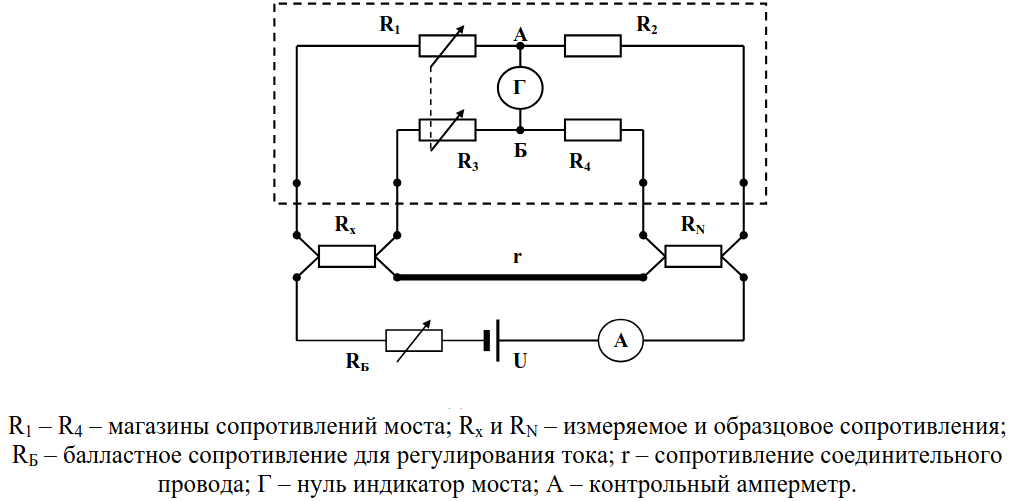
\includegraphics[scale=0.6]{scheme_2.png}
	\end{center}
	\caption{Мост Томпсона.}
\end{figure}

\section{Ход работы.}
\subsection{Задание 1. Мост Уитстона.}
1. Здесь нужно было измерить (вообще говоря, уже подписанные) сопротивления на плате. Они совпадают!
2. Измерить сопротивление катушки в воде и воздухе. Сначала измерялось в воздухе, затем - в воде со льдом. Также нужно определить комнатную температуру по следующей зависимости:
\begin{equation}
    R(T) = R(T_0)*(1+4,3*10^{-3}(T-T_0))
\end{equation}
откуда, при температуре $T_0 = 1^{\circ}С$ имеем:
\begin{equation}
    T = \frac{\frac{R(T)}{R(T_0)} - 1}{4,3*10^{-3}} - 1
\end{equation}
и подставляя значения:
\begin{equation}
    T = \frac{\frac{358,4}{329,4} - 1}{4,3*10^{-3}} - 1 = 21,5^{\circ}С
\end{equation}

\clearpage
\subsection{Задание 2. Мост Томпсона.}
1. Здесь нужно было измерить сопротивления образцовых резисторов. Показания сошлись с номинальными, указанными на самих резисторах.
2. Нужно было измерить сопротивление медного провода, построить график зависимости сопротивления проводника от его длины R(l). А также рассчитать удельное сопротивление меди.

\begin{equation}
    \rho = \frac{RS_{ср}}{l} = \frac{\pi d_{ср}^2 R}{4l}
\end{equation}


\begin{table}[ht!]
    \centering
    \begin{tabular}{|l|}
    \hline
        d, мм\\ \hline
        2    \\ \hline   
        1,97 \\ \hline
        1,94 \\ \hline
        1,96 \\ \hline
        2,01 \\ \hline
        2,03 \\ \hline
        2    \\ \hline
        1,96 \\ \hline
        1,98 \\ \hline
    \end{tabular}
    \caption{Диаметр проволоки}
\end{table}
Откуда $d_{ср} = 1,98$ мм.

\begin{table}[!ht]
    \centering
    \begin{tabular}{|l|l|l|}
    \hline
        $l$, м & $R$, ом & $\rho, \frac{Ом*мм^2}{м}$ \\ \hline
        0,4 & 0,00225 & 0,017 \\ \hline
        0,35 & 0,002 & 0,018 \\ \hline
        0,3 & 0,00169 & 0,017 \\ \hline
        0,25 & 0,0014 & 0,017 \\ \hline
        0,2 & 0,00107 & 0,017 \\ \hline
    \end{tabular}
\end{table}
\clearpage

\begin{figure}[ht!]
	\begin{center}
		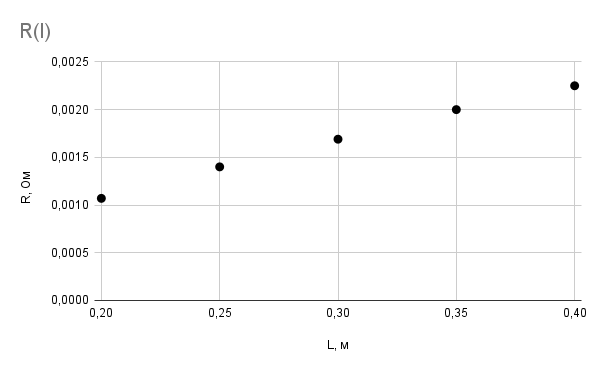
\includegraphics[scale=0.6]{R(l).png}
	\end{center}
	\caption{Зависимость R(l).}
\end{figure}

Из графика видно, что сопротивление линейно зависит от длины проводника. Собственно, это известно и из формулы (6).

\end{document}
